% kelompok 2 TUGAS 3 GIS (Database Access)
%Tiara Rizki Wulansari (1154026)
%Mohammad Agung Deomartha (1154032)
%M.Fajri Mualim (1154078)
%Faisal Syarifuddin (1154104)
%Muhamad Rifan Zamaludin (1154088)

\section {Database Access}

\subsection {Pengertian Database}
	Basis data adalah sekumpulan dari data yang telah disusun sesuai dengan aturan tertentu yang saling berhubungan sehingga memudahkan pengguna dalam mengelolanya juga memudahkan pengguna untuk memperoleh informasi. Selain itu ada juga yang menyebutkan bahwa database sebagai kumpulan file,tabel,atau arsip yang saling terhubung yang disimpan dalam media elektronik.
	Istilah "basis data" berawal dari ilmu komputer. Meskipun kemudian artinya semakin luas , memasukkan hal-hal di luar bidang elektronika, artikel ini mengenai basis data komputer. Catatan yang mirip dengan basis data sebenarnya sudah ada sebelum revolusi industri yaitu dalam bentuk buku besar, kuitansi dan kumpulan data yang berhubungan dengan bisnis.
	Jadi Database dapat disimpulkan adalah kumpulan informasi yang berkaitan dengan subjek atau tujuan tertentu , seperti pelacakan pesanan pelanggan atau menyimpan koleksi musik. Jika database tidak disimpan di komputer, atau hanya bagian dari dokumen tersebut, Anda dapat melacak semua jenis informasi dari berbagai sumber yang harus diseimbangkan dan ditata .

\subsection {Manfaat Penggunaan Database}
	\begin{enumerate}
		\item Kecepatan dan Kemudahan
		      Database memiliki kemampuan dalam menyeleksi data sehingga menjadi suatu kelompok yang tersusun dengan cepat. Hal inilah yang akhirnya dapat menghasilkan informasi yang dibutuhkan secara cepat pula. Seberapa cepat pemrosesan data oleh database tergantung pada perancangan databasenya.
     
		\item Pemakaian Bersama-sama
		      Suatu database bisa digunakan oleh siapa saja dalam suatu perusahaan. Sebagai contoh database mahasiswa dalam suatu perguruan tinggi dibutuhkan oleh beberapa bagian, seperti bagian admin, bagian keuangan, bagian akademik. Kesemua bidang tersebut membutuhkan database mahasiswa namun tidak perlu masing-masing bagian membuat databasenya sendiri, cukup database mahasiswa satu saja yang disimpan di server pusat. Nanti aplikasi dari masing-masing bagian bisa terhubung ke database mahasiswa tersebut. 
			
		\item Kontrol data terpusat 
		      Masih berkaitan dengan point ke dua, meskipun pada suatu perusahaan memiliki banyak bagian atau divisi tapi database yang diperlukan tetap satu saja. Hal ini mempermudah pengontrolan data seperti ketika ingin mengupdate data mahasiswa, maka kita perlu mengupdate semua data di masing-masing bagian atau divisi, tetapi cukup di satu database saja yang ada di server pusat. 
		
		\item Menghemat biaya perangkat
		      Dengan memiliki database secara terpusat maka di masing-masing divisi tidak memerlukan perangkat untuk menyimpan database berhubung database yang dibutuhkan hanya satu yaitu yang disimpan di server pusat, ini tentunya memangkas biaya pembelian perangkat.
 
		\item Keamanan Data 
		      Hampir semua Aplikasi manajemen database sekarang memiliki fasilitas manajemen pengguna. Manajemen pengguna ini mampu membuat hak akses yang berbeda-beda disesuaikan dengan kepentingan maupun posisi pengguna. Selain itu data yang tersimpan di database diperlukan password untuk mengaksesnya. 
		      
		\item Memudahkan dalam pembuatan Aplikasi baru 
		      Dalam poin ini database yang dirancang dengan sangat baik, sehingga si perusahaan memerlukan aplikasi baru tidak perlu membuat database yang baru juga, atau tidak perlu mengubah kembali struktur database yang sudah ada. Sehingga Si pembuat aplikasi atau programmer hanya cukup membuat atau pengatur antarmuka aplikasinya saja.
	\end{enumerate}

	Dengan segudang manfaat dan kegunaan yang dimiliki oleh database maka sudah seharusnya semua perusahaan baik itu perusahaan skala kecil apalagi perusahaan besar memiliki database yang dibangun dengan rancangan yang baik. Salah satu manfaat database adalah untuk memudahkan dalam mengakses data.Kemudahan pengaksesan data ini adalah sebagai implikasi dari keteraturan data yang
merupakan syarat mutlak dari suatu database yang baik. Ditambah dengan pemanfaatan teknologi jaringan komputer maka manfaat database ini akan semakin besar. Penggunaan database sekaligus teknologi jaringan komputer telah banyak digunakan oleh berbagai macam perusahaan,contohnya saja perbankan yang memiliki cabang di setiap kotanya. Perusahaan Bank tersebut hanya memiliki satu database yang disimpan di server pusat, sedangkan cabang-cabangnya terhubung melalui jaringan komputer untuk mengakses database yang terletak di sever pusat tersebut.


\subsection {Pengertian Character}
	Charakter merupakan bagian data yang terkecil, dapat berupa karakter numerik, huruf ataupun karakter-karakter khusus (special characters) yang membentuk suatu item data atau field.

\subsection {Apa yang dimaksud dengan Field, Record, Table, File, Data dan Basisdata} 
	Field merupakan kumpulan dari karakter yang membentuk satu arti, maka jika terdapat field misalnya seperti KeteranganBarang atau JumlahBarang, maka yang dimunculkan dalam field tersebut harus yang berkaitan dengan keterangan barang dan jumlah barang. Atau field juga bisa disebut sebagai tempat atau kolom yang terdapat dalam suatu tabel untuk mengisikan nama-nama (data) field yang akan di isikan. merepresentasikan suatu atribut dari record yang menunjukkan suatu item dari data, seperti misalnya nama, alamat dan lain sebagainya. Kumpulan dari field membentuk suatu record.

	Record merupakan kumpulan field yang sangat lengkap, dan biasanya dihitung dalam satuan baris. Tabel merupakan kumpulan dari beberapa record dan juga field. 
	
	File terdiri dari kumpulan field yang menunjukan dari satu kesatuan data yang sejenis. Misalnya seperti file nama siswa berisikan data tentang semua nama siswa yang ada. Data adalah kumpulan fakta atau kejadian yang digunakan sebagai penyelesaian masalah dalam bentuk informasi. Basis data (database) terdiri dari dua kata, yaitu kata basis dan data. Basis merupakan tempat ataupun gudang, ataupun wadah.

	Data dapat disebut sebagai kumpulan dari fakta yang mewakili objek, misalnya seperti benda, manusia,barang dan sebagainya yang ditulis ke dalam bentuk angka, huruf, simbol, bunyi, teks, gambar ataupun gabungannya. Jadi dapat disimpulkan bahwa basis data merupakan kumpulan dari data-datayang terorganisasi yang saling berhubungan sedemikian rupa sehingga dapat dengan mudah disimpan, dimanipulasi, dan dipanggil oleh pemakainya. Karakter atau character yang ada didalam database merupakan bagian data yang terkecil, karakter tersebutdapat berupa karakter numerik, huruf ataupun karakter khusus (special characters) yang membentuk suatu item data atau field.

\subsection {Sifat-sifat database atau basis data}
	Data dalam basis data bersifat integrated dan shared Terpadu (integrated), berkas-berkas data yang ada pada basis data saling terkait (terjadi dependensi data);
	Berbagi data (shared), data yang sama dapat dipakai oleh sejumlah pengguna dalam waktu yang bersamaan. Sering dinamakan sebagi sistem multiuser.
	\begin{itemize}
		\item Internal : Kesatuan (integritas) dari file-file yang terlibat
		\item Terbagi atau share : Elemen-elemen database dapat dibagikan pada para user baik secara sendiri-sendiri maupun secara serentak dan pada waktu yang sama (concurrent sharing).
	\end{itemize}
 
\subsection {Tipe Database} 
	Tipe Database Terdapat 12 tipe database, antara lain: 
	\begin{enumerate}
		\item Operational database: Database ini menyimpan data rinci yang diperlukan untuk mendukung operasi dari seluruh organisasi. Mereka juga disebut subject-area databases (SADB), transaksi database, dan produksi database. Contoh: database pelanggan, database pribadi, database inventaris, akuntansi database.
 
		\item Analytical database: Database ini menyimpan data dan informasi yang diambil dari operasional yang dipilih dan eksternal database. Mereka terdiri dari data dan informasi yang dirangkum paling dibutuhkan oleh sebuah organisasi manajemen dan End-user lainnya. Beberapa orang menyebut analitis multidimensi database sebagai database, manajemen database, atau informasi database.

		\item Data warehouse: Sebuah data warehouse menyimpan data dari saat ini dan tahun- tahun sebelumnya - data yang diambil dari berbagai database operasional dari sebuah organisasi.

		\item Distributed database: Ini adalah database-kelompok kerja lokal dan departemen di kantor regional, kantor cabang, pabrik-pabrik dan lokasi kerja lainnya. Database ini dapat mencakup kedua segmen yaitu operasional dan user database, serta data yang dihasilkan dan digunakan hanya pada pengguna situs sendiri. 
 
		\item End-user database: Database ini terdiri dari berbagai file data yang dikembangkan oleh end-user di workstation mereka. Contoh dari ini adalah koleksi dokumen dalam spreadsheet, word processing dan bahkan download file. 

		\item External database: Database ini menyediakan akses ke eksternal, data milik pribadi online - tersedia untuk biaya kepada pengguna akhir dan organisasi dari layanan komersial. Akses ke kekayaan informasi dari database eksternal yang tersedia untuk biaya dari layanan online komersial dan dengan atau tanpa biaya dari banyak sumber di Internet.

		\item Hypermedia databases on the web: Ini adalah kumpulan dari halaman-halaman multimedia yang saling berhubungan di sebuah situs web. Mereka terdiri dari home page dan halaman hyperlink lain dari multimedia atau campuran media seperti teks, grafik, gambar foto, klip video, audio dll. 

		\item Navigational database: Dalam navigasi database, queries menemukan benda terutama dengan mengikuti referensi dari objek lain.
 
		\item In-memory databases: Database di memori terutama bergantung pada memori utama untuk penyimpanan data komputer. Ini berbeda dengan sistem manajemen database yang menggunakan disk berbasis mekanisme penyimpanan. Database memori utama lebih cepat daripada dioptimalkan disk database sejak Optimasi algoritma internal menjadi lebih sederhana dan lebih sedikit CPU mengeksekusi instruksi.

		\item Document-oriented databases: Merupakan program komputer yang dirancang untuk aplikasi berorientasi dokumen. Sistem ini bisa diimplementasikan sebagai lapisan di atas sebuah database relasional atau objek database. Sebagai lawan dari database relasional, dokumen berbasis database tidak menyimpan data dalam tabel dengan ukuran seragam kolom untuk setiap record. Sebaliknya, mereka menyimpan setiap catatan sebagai dokumen yang memiliki karakteristik tertentu. Sejumlah bidang panjang apapun dapat ditambahkan ke dokumen. Bidang yang dapat juga berisi beberapa bagian data. 
 
		\item Real-time databases Real-time: Database adalah sistem pengolahan dirancang untuk menangani beban kerja negara yang dapat berubah terus- menerus. Ini berbeda dari database tradisional yang mengandung data yang terus- menerus, sebagian besar tidak terpengaruh oleh waktu. 
 
		\item Relational Database: Database yang paling umum digunakan saat ini. Menggunakan meja untuk informasi struktur sehingga mudah untuk mencari.
	\end{enumerate}
 
 
\subsection {Modul python untuk mengakses database MySQL}
	Untuk mengakses database MySQL dari Python, berikut adalah beberapa langkah sederhana. Yang pertama, server database MySQL harus siap dulu. Karenanya lakukan tahapan berikut ini. 
	\begin{enumerate}
		\item Instal server mysql dengan menjalankan perintah sudo apt-get install mysqlserver. Jangan lupa memasukkan password akun root untuk server MySQL. 
		\item Siapkan database dan tabel. Jalankan perintah mysql -u root -p dari terminal. 
			Selanjutnya kita akan buat tabel yang skemanya seperti berikut ini (hanya ilustrasi saja).
			\begin{equation} 
			mysql> create database teman; 
			\end{equation}
			mysql> use teman; 
			mysql> create table alamat(id int not null auto increment primary key, 
			nama varchar(35), alamat text, telepon varchar(15), surat text);

		\item  ingin membuat user baru yang punya akses penuh ke database yang baru saja dibuat, lakukan tahapan berikut ini. 
			mysql> create user 'andri'@'localhost' identified by '123456'; 	
			mysql> grant all on teman.* to 'andri'@'localhost' with grant option; 

		\item Langkah selanjutnya adalah membuat modul python untuk mengakses database tersebut. Untuk kasus ini, modul hanya diberi kemampuan untuk melihat seluruh isi tabel, sehingga tabel sebaiknya diisi dulu. Sedangkan kemampuan untuk melakukan operasi update dan delete dapat dibangun menggunakan pola yang sama. Modul tersebut seperti code berikut. 
	\end{enumerate}

Dalam modul python ini terdiri dari dua fungsi, masing-masing sambung dan selectall. Fungsi pertama membutuhkan parameter terkait nama server, dan akun user serta mengembalikan variabel koneksi. Sedangkan fungsi selectall membutuhkan parameter koneksi yang diperoleh dari fungsi sambung, serta nama database dan nama tabel. Fungsi ini mengembalikan list yang berisi setiap row dalam tabel untuk kebutuhan lain yang belum terdefinisi dalam modul ini. Berikut Contoh selectall dalam python ;

	\begin{verbatim}
		def sambung (host,user,passwd): 
		mycon=MySQLdb.connect(host,user,passwd) 
		return mycon
		
		def selectall(mycon, dbname, table): 
		mycur=mycon.cursor() 
		mycur.execute(’use ’ + dbname) 
		mycur.execute(’select * from ’ + table) 
		rows=mycur.fetchall() 
		a=[] 
		for i in rows: 
		nama=i[1] 
		alamat=i[2] 
		telepon=i[3] 
		surat=i[4] 
		print(nama + ’ ’ + alamat + ’ ’ + telepon + ’ ’ + surat) 
		a.append(i) 
		return a 
	\end{verbatim}

Lalu, bagaimana menggunakannya? Untuk sementara, modul python ini hanya dapat diakses melalui shell python karena belum ada fungsi main yang terdefinsi. Hal ini disebabkan karena rancangan input/ouput masih seadanya. Karenanya, mari masuk ke shell python dengan menjalankan perintah python di terminal. Yang perlu diperhatikan, penggunaan shell python harus dilakukan dari directory di mana modul ini disimpan. Berikut adalah gambaran ketika berada dalam shell python dan menggunakan modul ini. 

	\begin{verbatim}
		>>> from mymodul import * 
		>>> mycon=sambung(”localhost”,”andri”,”123456”) 
		>>> a=selectall(mycon,”teman”,”alamat”) 
		Andri Jl. Sariasih, Sarijadi, Bandung 12450 08123456789 andri@poltekpos.ac.id 
		>>> 
	\end{verbatim}
	
Di baris pertama, kita import modul dari nama file, untuk selanjutnya import semua fungsi yang ada di dalamnya. Selanjutnya, kita membuat variabel bernama mycon bertipe koneksi ke MySQL (dapat dilihat dengan cara menjalankan perintah type(mycon) dari shell python) dan meng-assigned nilainya dari memanggil fungsi sambung. Selanjutnya, variabel a di-assinged nilainya dari memanggil fungsi selectall. Terlihat bahwa fungsi selectall mencetak nilai yang diperoleh dari operasi select tabel. 

Dengan ilustrasi ini, diharapkan dapat memberi inspirasi dalam membuat modul python yang digunakan untuk sebuah aplikasi, misalnya dengan menjadikannya sebagai bagian dari hubungan SIGNAL-SLOT pada QT4. Semoga bermanfaat. 

Dalam era informasi dimana kita hidup sekarang, kita dapat melihat seberapa banyak data dunia berubah. Kita pada dasarnya membuat, menyimpan, dan menarik data, secara ekstensif. Harusnya ada sebuah cara untuk menangani semua itu. Semua itu tidak dapat disebarkan kemana-mana tanpa adanya manajemen bukan? Di sini hadir Database Management System (DBMS). DBMS adalah sebuah sistem software yang memungkinkanmu untuk membuat, menyimpan, memodifikasi, menarik, dan penanganan lainnya terhadap sebuah data dari database. Sistem ini juga bervariasi dalam ukuran, mulai dari sistem kecil yang cukup berjalan pada komputer personal hingga yang lebih besar yang berjalan dalam mainframe. 

\subsection {Python Database API} 
	Python dapat berinteraksi dengan database. Namun, bagaimana cara melakukannya? Python menggunakan apa yang disebut Python Database API dengan tujuan untuk menjadi antarmuka dengan database. API ini mengijinkan kita untuk memprogram database management system (DBMS) yang berbeda. Untuk DBMS yang berbeda itu, bagaimana pun juga, proses yang diikuti pada tingkatan kode tetap sama, yaitu sebagai berikut: 
	\begin{enumerate}
		\item Membangun sebuah koneksi ke database pilihanmu. Kita bisa membuat function koneksi, kemudian dipanggil dari file atau script atau halaman lain. Hanya menyediakan fungsi koneksi saja. 
		\item Kita membuat class koneksi, kemudian dipanggil dari file atau script atau halaman lain.
Menyediakan fungsi-fungsi dasar eksekusi perintah ke database seperti execute, mengambil data dan lainnya.
		\item Memanipulasi data menggunakan SQL (berinteraksi). 
		\item Memberitahu koneksi untuk entah menerapkan manipulasi SQL ke data dan membuatnya permanen (commit), atau memberitahunya untuk meninggalkan manipulasi itu (rollback), sehingga mengembalikan data ke keadaan sebelum interaksi terjadi. 
		\item Kita membuat library php yang isinya koneksi kemudian tinggal pakai dalam aplikasi. Menyediakan fitur-fitur lengkap tentang koneksi ke database, bahkan menyediakan berbagai pilihan jenis database.
	\end{enumerate}
	
Bagaimana caranya menampilkan data dari mysql menggunakan python. Saya asumsikan teman-teman sudah menginstall web server (XAMPP/yang lainnya) dan python di komputer masing-masing. Setelah itu semua siap sekarang silahkan download mysql connector untuk python disini (Sesuaikan dengan versi python yang kalian punya). Setelah itu tinggal install. Setelah selesai installasi, buka phpmyadmin dan buat database dengan nama terserah. Contohnya yaitu trial Lalu import sql berikut
	trial.sql 
	Setelah di impor, lalu buka teks editor dan copas-kan code berikut 
	show-data.py 
	lalu simpan dengan nama terserah kalian (punya saya show-data.py) dan tinggal 
	kalian run dari command prompt. 

\subsection {Koneksi Database MySQL dengan Python}
	\begin{enumerate}
		\item  Pastikan kita sudah menginstal package libmysqlclient-dev dengan sebagai berikut: 
		       apt-get install libmysqlclient-dev 
		\item  Download modul MySQLdb.
		\item  Instal modul tersebut ini dengan cara (Pastikan saat login sebagai root ya):
	    \begin{verbatim}
			$ gunzip MySQL-python-1.2.2.tar.gz 
			$ tar -xvf MySQL-python-1.2.2.tar 
			$ cd MySQL-python-1.2.2 
			$ python setup.py build 
			$ python setup.py install 
		\end{verbatim}
		\item  Buat sebuah script seperti berikut (dengan contoh: test.py):
		    \begin{verbatim}
			import MySQLdb 
			# Open database connection 
			db = MySQLdb.connect(”localhost”,”root”,”password”,”nama database” ) 
			# prepare a cursor object using cursor() method 
			cursor = db.cursor() 
			# execute SQL query using execute() method. 
			cursor.execute(”SELECT VERSION()”) 
			# Fetch a single row using fetchone() method. 
			data = cursor.fetchone() 
			print ”Database version : %s ” % data 
			# disconnect from server 
			db.close()
			\end{verbatim}
		\item Test dengan code berikut:
		      python test.py 
	\end{enumerate}
	
\subsection {Connection Class}
	Metode ini menggunakan kelas untuk menginisialisasi koneksi pada database. Pada contoh ini hanya menggunakan kelas sebagai inisiator untuk menghubungkan ke database, untuk querynya tetap menggunakan metode biasa.
	\begin{enumerate}
		\item pertama kita membuat kelas koneksi, buatlah file koneksi dengan nama connection.py dan masukan coding berikut :
			\begin{verbatim}
			import MySQLdb as mysql
			import hashlib
			import sys
			import warnings
			class MysqlUserDB:
    			# initialization Connection Database
    			# Init Start
    			warnings.filterwarnings('error')
    			def __init__(self, DBrootHost, DBrootUser, DBrootPass, DBrootDatabase):
        		self.DBrootHost = DBrootHost
        		self.DBrootUser = DBrootUser
        		self.DBrootPass = DBrootPass
        		self.DBrootDatabase = DBrootDatabase
        		try:
            		print("Checking connection of MYSQL ...")
            		self.con = mysql.connect(DBrootHost, DBrootUser, DBrootPass, DBrootDatabase)
            		self.cursor = self.con.cursor()
            		self.cursor.execute('Select version()')
            		print("Connected to Mysql Database\n")
        		# except mysql.Error as error:
        		#    print("Error %s\n Stop.\n" % error)
        		#    sys.exit()
        		except Warning as warn:
            		print("Warning", warn)
    			def CreateDB(self, DBrootDatabase):
        		print("Creating database...")
        		try:
            		self.cursor.execute('CREATE database if NOT exists ' + DBrootDatabase)
            		self.cursor.execute("SHOW DATABASES LIKE %s", (DBrootDatabase,))
            		dbs = self.cursor.fetchone()
            		print("Database created: ", dbs[0])
        		except Warning as warn:
            		print("Warning: %s \nStopping Process.\n" % warn)
            		sys.exit()
    			def GrantsAccess(self, DBrootDatabase):
        		print("Accessing Account ...")
        		try:
            		self.cursor.execute("SHOW DATABASES LIKE %s", (DBrootDatabase,))
            		result = self.cursor.fetchone()
            		print("Access Granted for Database", result[0])
        		except Warning as warn:
            		print("Warningg %s" % warn)
    			def getDB(self):
        		return self.cursor
    			def delCon(self):
        		print("Finishing operation ...")
        		self.cursor.close()
        		self.con.close()
        		print("Finished")
			# Init End
		\end{verbatim}

Dalam kelas fungsi diatas menginisialisasi paramater untuk koneksi yang dinisialisasi pada method init, 
Sedangkan untuk me-return hasil koneksi menggunakan method getDB hal ini untuk mereturn cursor untuk dipanggil saat akan melakukan eksekusi, dan untuk memutuskan koneksi menggunakan method delcon, sedangkan sisa method lainnya hanya sebagai method pendukung.
	
	\item Setelah itu, buatlah file baru untuk mengetes apakah koneksi berhasil dan melakukan query.
buatlah file menggunakan nama connectionTes.py
		\begin{verbatim}
			import connection as dbs
			import warnings
			warnings.filterwarnings('error')
			mysqli = dbs.MysqlUserDB(DBrootHost='127.0.0.1', DBrootUser='root',
        	                 DBrootPass='', DBrootDatabase='pos')
			db = mysqli.getDB()
			try:
    			db.execute("select * from product")
    			results = db.fetchall()
    			for result in results:
        		print(result)
			except db.Error as error:
	   		print(error)
			mysqli.delCon()
		\end{verbatim}
    \end{enumerate}
Dalam hal ini mengimport kelas connection sebagai db. Setelah itu di inisialisasi dengan variabel baru bernama mysqli.
dan membuat object cursor pada db dengan memanggil object kelas mysql.getDB()

\begin{table}[ht]
	\caption{Arsitektur Database}
	\centering
	\begin{tabular}{cccc}
		\hline
		No&Keterangani&\\
		\hline
		.1&Database Connection&\\
		.2&SQL Statements&\\
		.3&Result Set&\\
		.4&Database Metadata&\\
		.5&Prepared Statement\\
		\hline
	\end{tabular}
\end{table}

\ref{DA.png}:
\begin{figure}[ht]
	\centerline{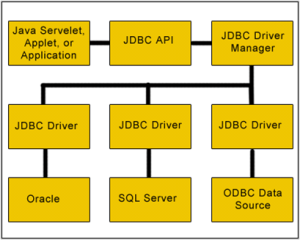
\includegraphics[width=0.70\textwidth]{figures/DA.png}}
	\caption{Arsitektur}
	\label{DA.png}
\end{figure}
